\section{Methodology}
\label{section:method}
In this section, we present our meta-heuristic-based methodology for image contrast enhancement. Meta-heuristic methods share several common features~\cite{glover2003handbook}. Each method begins with an initial set of {\em individuals}, often referred to as the {\em population}. To introduce diversity into the population, special operations, known as {\em mutations}, are applied to generate new populations. In each iteration, the fittest individuals are selected based on a mathematical function known as the {\em fitness function}. This process of generating new population is repeated for a fixed number of iterations, with the fittest population from all iterations is considered the best solution found. While this approach does not guarantee an optimal solution, it is effective at discovering {\em good} solutions within a relatively short time frame. However, the difference between most meta-heuristics algorithms lies in the way in which the initial population is generated and the mutation function is applied. 

At a high level, we employed Hill Climbing and Genetic Algorithm-based techniques, exploring five different variants of these approaches. Specifically, we implemented three variants of Hill Climbing and two variants of the Genetic Algorithm. For the Hill Climbing approach, the variants differ in their mutation functions and input membership functions, as detailed below. For the Genetic Algorithm, we used a single type of input membership function, with variations in the next generation selection strategies (see Section \ref{subsection:method_ga_join}).
% \begin{itemize}
%     \item Hill Climbing
%         \begin{enumerate}
%             \item neighborhood generation using simple mutation
%             \item neighborhood generation with Trapezoidal and triangular input membership set splitting mutation
%             \item mixed neighborhood generation with Gaussian input membership set splitting mutation
%         \end{enumerate}
%     \item Genetic Algorithm
%     \begin{enumerate}
%             \item simple neighborhood generation with Trapezoidal and Triangular input membership set
%             \item simple neighborhood generation with Gaussian and Sigmoid input membership set
%         \end{enumerate}
% \end{itemize}
First, we discuss the subroutines that are common among all variants of metaheuristics approaches, namely, initialization, representation, and fitness assessment. 
\begin{figure}
    \centering
    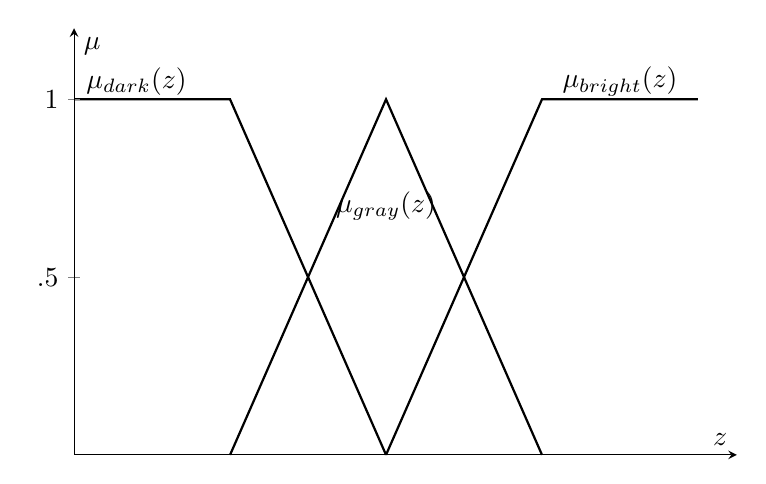
\begin{tikzpicture}
        \begin{axis}[
            axis lines=middle,
            xlabel={$z$},
            ylabel={$\mu$},
            ymin=0, ymax=1.2,
            xmin=0.0, xmax=8.5,
            xtick=\empty,
            ytick={0, 0.5, 1},
            yticklabels={0, .5, 1},
            width=10cm,
            height=7cm,
            enlargelimits=false,
            axis on top,
            clip=false,
            domain=-1:8
            ]
    
            % Dark membership function
            \addplot[thick] coordinates {(0,1) (2,1) (4,0)};
    
            % Gray membership function
            \addplot[thick] coordinates {(2,0) (4,1) (6,0)};
    
            % Bright membership function
            \addplot[thick] coordinates {(4,0) (6,1) (8,1)};
    
            % Labels
            \node at (axis cs: 0.8, 1.05) {$\mu_{\text{dark}}(z)$};
            \node at (axis cs: 4, 0.7) {$\mu_{\text{gray}}(z)$};
            \node at (axis cs: 7, 1.05) {$\mu_{\text{bright}}(z)$};
    
        \end{axis}
    \end{tikzpicture}
    \caption{Input membership functions for fuzzy, rule-based contrast enhancement  \cite{gonzalez2008digital}}
    \label{fig:fuzzy_function}
\end{figure}
% \begin{figure}
%     \centering
%     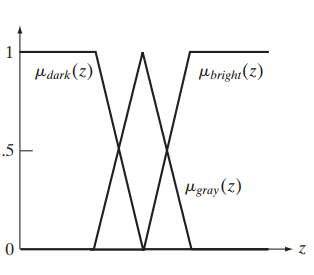
\includegraphics[scale=0.8]{fuzzy_function.PNG}

% \end{figure}


%\subsection*{Population Initialization}
\subsection{Population Representation}
\label{subsection:method_pop}
Every meta-heuristics technique starts with some (usually randomly generated) initial population and the structure of the population is specific to the problem we are aiming to solve. In our case, each candidate is an input membership function, as shown in Figure \ref{fig:fuzzy_function}. So, our population representation holds information about a set of input membership functions. Within each input membership function, there are at least three functions. Each membership function is represented by a tuple of three values regardless of the function types (i.e., trapezoidal, triangular, Gaussian, and Sigmoidal). The first two values of the tuple determine the shape of the membership function, and the third one is used in defuzzification.

\subsection{Fitness Assessment}
\label{subsection:fitness_assessment}
Following the literature of image enhancement~\cite{munteanu2004gray}, we calculate an individual's ($I$) quality/fitness using the following fitness function: 
%There are some terms in Equation \ref{eqn:fitness} which we will explain now, 
\begin{equation} \label{eqn:fitness}
\fitness{I} = \log{\log{\intensity{I_s}}} \times \frac{\edge{I_s}}{M \times N} \times \entropy{I_s}
\end{equation}
\begin{description}
    \item[$I_s$] $=$ image after Applying {\em Sobel filter} on $I$
    \item[$\intensity{I}$] $=$ sum of intensity of image $I$
    \item[$\edge{I}$] $=$ number of edge pixel in $I$
    \item[$\entropy{I}$] $=$ entropy of image $I$
    \item[$M$] $=$ width of $I$
    \item[$N$] $=$ height of $I$
\end{description}

\subsection*{HSV Conversion}
\label{subsection:method_hsv}
If the input image is a color image, we need to convert it to the HSV format. In the case of a gray-scale image, there is no need for such a conversion. 

\subsection*{Defuzzification}
\label{subsection:method_defuzz}
Defuzzification refers to converting the fuzzy value to a {\em single crisp} value. For any given input pixel $z_0$, the output crisp value $v_0$ will be as follows.
\begin{equation} \label{eqn:defuzzy}
v_0 = \frac{\sum\limits_{i=1}^n\mu_{i}(z_0) * v}{\sum\limits_{i=1}^n\mu_{i}(z_0)};n\geq3
\end{equation}
Here,
\begin{description}
    \item[$\mu_{i}(z_0) = $] \quad fuzzy level of the image pixel with value $z_0$
    \item[$v =$] constant/mutable value (depending on the algorithm variant) used in the defuzzification 
\end{description}

\subsection{Hill Climbing}
\label{subsection:method_hc}
The Hill Climbing technique stochastically generates new individuals and stores the fittest individual as the candidate solution. The best solution is evaluated using the fitness function shown in Equation \ref{eqn:fitness}. In each generation, we generate a certain number of neighbor solutions (set to $10$) from a fixed individual. We have tried three variants of Hill Climbing differing from each other in neighborhood generation and input membership function type.

\subsubsection{Simple Neighborhood Generation}
\label{subsubsec:simple_neighbour_generation}
In this variant, we have initiated an individual with two trapezoidal ($\mu\_dark, \mu\_bright$) and one triangular ($\mu\_gray$) functions like Figure \ref{fig:fuzzy_function}. 
When generating a new individuals, only the shapes of the functions (i.e., the width of the triangle and trapezoid's oblique line's slope) are tweaked. 
We have adapted three hyperparameters, namely, $\mathsf{ChangeProb}$, $\mathsf{MutateMu}$, and $\mathsf{MutateSigma}$. 
Firstly, $\mathsf{ChangeProb}$ represents the threshold of the random number chosen to decide whether the shape change will be performed or not. 
On the other hand, $\mathsf{MutateMu}$ and $\mathsf{MutateSigma}$ represent, respectively, the mean and variance of Gaussian distribution from which the random number is chosen when generating a new solution. 
% no need ===
% \subsubsection*{Neighborhood Generation with trapezoidal and triangular input membership set splitting mutation}
% \label{subsubsection:method_hc_traptri_split}
% This variant considers an additional tweak besides the previous one. A membership function may split into two membership functions (e.g., one triangle in Figure \ref{fig:fuzzy_function} splits into two). In addition to the previously mentioned parameters, here we have used another one, which is $\mathsf{MembershipSplitProb}$, to control the probability of choosing function shape change or input member function splitting.
% \subsubsection*{Neighborhood Generation with Gaussian input membership set splitting mutation}
% \label{subsubsection:method_hc_gauss_split}
% In this case, we have used only the Gaussian input membership function in our solution. All the hyperparameters mentioned in the previous two cases are used.

\subsection{Genetic Algorithm}
\label{subsection:method_ga}
Unlike Hill Climbing, the Genetic Algorithm (GA) starts with a number (say, $\mathsf{PopSize}$) of individuals. We use the same evaluation function shown in Equation \ref{eqn:fitness} for fitness evaluation in our GA approach. To introduce variations in the population, GA breeds a new population of children, selects individuals from the old population, and tweaks them to breed new individuals. To keep the footprints of both populations, it joins the parent and children populations to form a new generation of population. In our implementation, we have fixed $\mathsf{PopSize}$ equal to $30$.

\subsection{Tweaking Operations}
\label{subsection:method_ga_tweak}
\subsubsection{Crossover}
The crossover operation mixes multiple individuals (typically $2$) and matches to form the children. There are $3$ classical ways of doing a crossover. In our implementation, we have used {\em uniform crossover}. In the context of our representation, our crossover operation marches down all the membership functions and to combine them swaps individual functions if a coin toss comes up head with probability $p$. To use crossover on the Genetic Algorithm, both individuals should be of the same size. 

\subsubsection{Mutation}
\label{subsection:method_ga_mut}
Our mutation operation scans each membership function and randomly tweaks the function shape with a certain probability. To exploit both exploitation and exploration, our mutation operation uses a Gaussian distribution with a certain mean and variance. 
% Unlike Hill Climbing, mutation operation here does not increase/decrease the number of membership functions.

\subsection{Joining}
\label{subsection:method_ga_join}
The Genetic Algorithm differs in how parent and child populations are joined. In our Genetic Algorithm procedure, we have experimented with both $(P, P)$ and $(P+P)$ evolution strategies, where $P$ is the $\mathsf{PopSize}$.

% \subsection{Experiment Process}
% \label{subsection:experiment_process}
% In the experimental analysis, first, we choose the best variants among all variants of Hill Climbing and the Genetic Algorithm. Then we measure the performance of our image enhancement method with respect to common metrics of image enhancements, and finally, we compare our results with one of the simplest methods of image enhancement --- histogram equalization.
% %The objective of our experiment is first select the best two variants from the five variants we have experimented on, then we have measured different metrics of the output images to compare them with a simple contrast enhancement approach called histogram equalization.

% \subsubsection{Variant Selection}
% The following steps are used to choose the best variants:

% \begin{enumerate}
%     \item Run one variant on each image. The variant is applied on one image a total of $\mathsf{NumofTest}$ times. Each time (one stochastic optimization) is run for $ \mathsf{PerRunTime}$ seconds. This time is kept the same for all variants. Also, mutation and population initialization-related parameters are kept the same for all variants. 
%     %(except $SPLIT\_PROB$ because variants are also differentiated based on this).  
    
%     \item Measure the average rate of fitness improvement over the number of generations achieved in given $\mathsf{PerRunTime}$. Then the average is computed for $\mathsf{NumofTest}$ times.
    
%     \item We have compared the metric achieved in step $2$ for all five variants and then selected the best two variants. The higher the value of this metric demonstrates better performance.
% \end{enumerate}

The value of experiment controlling parameters is written in Table \ref{tab:exp_parameters}.

\begin{table}[]
    \centering
    \begin{tabular}{| c | c |}
        \hline
        \textbf{Hyperparameter name} & \textbf{Value}\\
        \hline
        $\mathsf{NumofTest}$ & $5$ \\ 
        \hline
        $\mathsf{PerRunTime}$ & $120$ \\
        \hline
        $\mathsf{ChangeProb}$ &  $0.5$\\
        \hline
        $\mathsf{MutateMu}$ & $3$ \\
        \hline
        $\mathsf{MutateSigma}$ & $2$ \\
        \hline
        $\mathsf{MembershipSplitProb}$ & $0.1$ \\
        \hline
    \end{tabular}
    \caption{The value of hyperparameters}
    \label{tab:exp_parameters}
\end{table}

 







